%----------------------------------------------------------------------------------------
%	PACKAGES AND THEMES
%----------------------------------------------------------------------------------------
\documentclass[aspectratio=169,xcolor=dvipsnames]{beamer}

\usepackage{hyperref}
\usepackage{graphicx} % Allows including images
\usepackage{booktabs} % Allows the use of \toprule, \midrule and \bottomrule in tables
\usepackage{bm}% bold math
\usepackage{physics}
\setlength{}{}%
\usepackage{siunitx}
\usepackage[inline]{asymptote}
\usepackage{multirow}
\usepackage{tikz}
\usetikzlibrary{shapes,arrows, positioning}

\usepackage{pgfplots, pgfplotstable}
\pgfplotsset{compat=1.16}
\usepackage{hyperref}
\usepackage{natbib}
% \usepackage{amsthm}
\usepackage{amssymb}
\usepackage{amsmath}
\usepackage{cancel}

% The title
\title[short title]{PHY372: All-Photonics Quantum Repeaters}
% \subtitle{Subtitle}

\author{QiLin Xue}
\institute[UofT] % Your institution may be shorthand to save space
{
    % Your institution for the title page
    University of Toronto
    \vskip 3pt
}
\date{\today} % Date, can be changed to a custom date


%----------------------------------------------------------------------------------------
%	PRESENTATION SLIDES
%----------------------------------------------------------------------------------------
\begin{document}
\begin{frame}
    \titlepage
\end{frame}
\begin{frame}
\frametitle{Motivation: Overview}
\begin{itemize}
    \item Current cryptography relies on unproven hardness of certain problems
    \item Quantum cryptography uses the laws of physics for unconditional security.
    \item \textbf{Challenge:} Channel loss and noise increase with distance.
\end{itemize}
\end{frame}

\begin{frame}
\frametitle{Classical vs Quantum Repeaters}
\begin{itemize}
    \item Classical repeaters amplify signals to overcome loss in transmission medium.
    \item Quantum signals cannot be amplified due to the \textbf{no cloning theorem.}
    \item Instead, create long-distance entanglement linking distant nodes through 'entanglement swapping'.
\end{itemize}
\begin{center}
    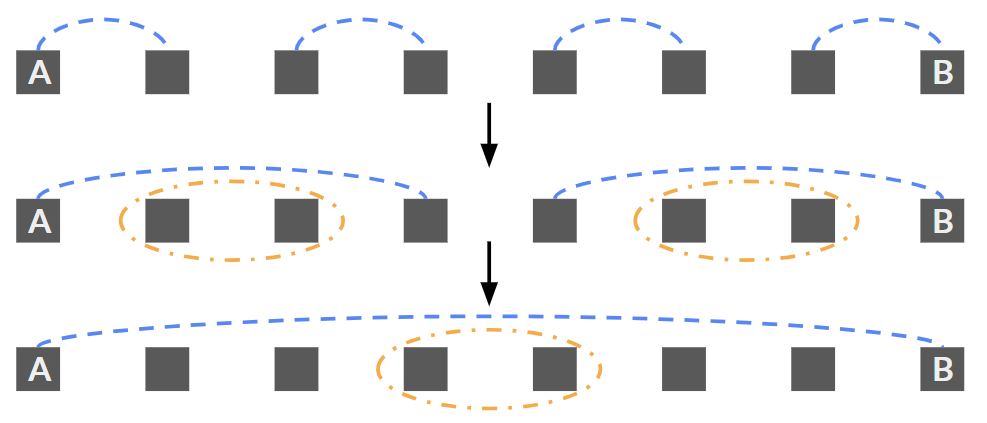
\includegraphics[width=0.7\linewidth]{figs/quantum-repeater.png}
\end{center}
\end{frame}
\begin{frame}
\frametitle{Challenges with Quantum Repeaters}
\begin{itemize}
    \item Quantum Memory
    \item Ability to convert between staionary and flying qubits
    \item $\implies$ Could be as hard as quantum computers!  
\end{itemize}    
\end{frame}
\begin{frame}
\frametitle{All-Photonics Quantum Repeater}
\begin{itemize}
  \item No need for quantum memory.
  \item Multiple channels for creating entanglement.
\end{itemize}
\begin{center}
    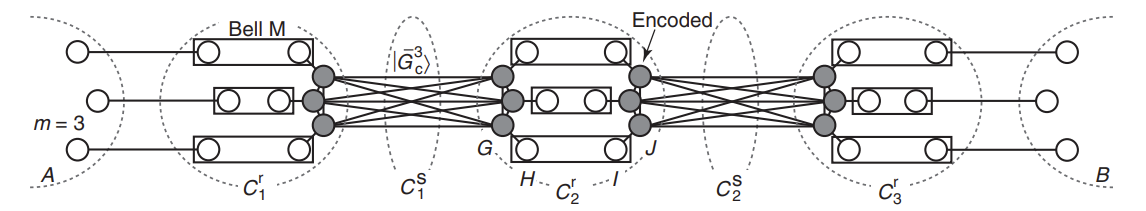
\includegraphics[width=\linewidth]{figs/photonics.png}
\end{center}
\end{frame}

\begin{frame}
    \frametitle{Overview of Photonic Quantum Repeaters}
    \begin{itemize}
        \item Two stages:
        \begin{center}
            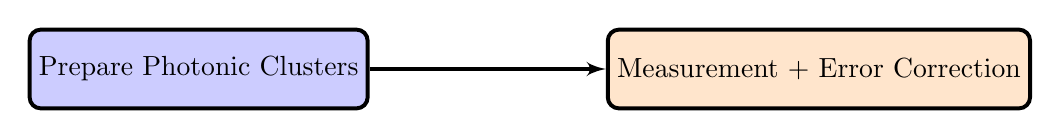
\begin{tikzpicture}[node distance=3cm,auto,>=latex',
                every node/.style={draw, scale=1, align=center, rectangle, rounded corners, minimum height=1cm, minimum width=2cm, line width=0.5mm},
                block/.style={fill=blue!20},
                correction/.style={fill=orange!20}
                ]
                \node[block] (init) {Prepare Photonic Clusters};
                \node[correction, right=3cm of init] (measure) {Measurement + Error Correction};
                \draw[->,line width=0.5mm] (init) -- (measure);
        \end{tikzpicture}
    \end{center}
    \item \textbf{Preparation:} Compute $P_{cn},$ the probability to prepare the clusters
    \item \textbf{Measurement:} Compute the key rate $R$ by looking at success probability of measurements.
\end{itemize}
\begin{center}
    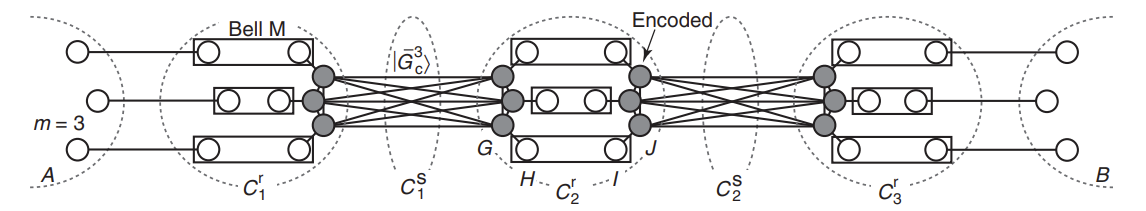
\includegraphics[width=\linewidth]{figs/photonics.png}
\end{center}
\end{frame}
\begin{frame}
    \frametitle{Building a Cluster State: Repeater Nodes}
    \begin{itemize}
        \item Attach error protection trees with branching vector $\vec{b}=[b_0, b_1].$ 
        \item White qubits are \textit{outer qubits} that are transmitted to receiver nodes.
    \end{itemize}
    \begin{center}
        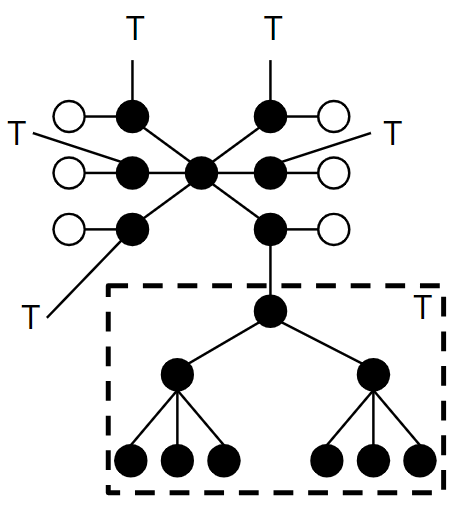
\includegraphics[width=0.3\linewidth]{figs/cluster.png}
    \end{center}
    In above example, $\vec{b}=[2,3]$ and $m=3.$
\end{frame}
\begin{frame}
    \frametitle{Building a Cluster State: Repeater Nodes}
    \begin{itemize}
        \item $4m+1$ basis measurements are done to turn tree into a cluster
        \item Allows for maximal error correction
    \end{itemize}
    \begin{center}
        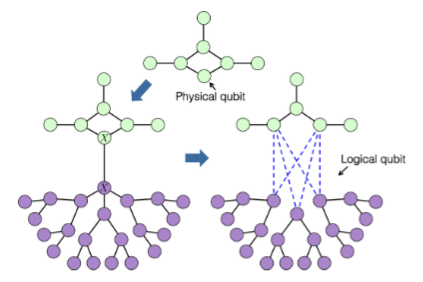
\includegraphics[width=0.5\linewidth]{figs/measurement.png}
    \end{center}
    \end{frame}
\begin{frame}
\frametitle{Building a Cluster State: Fusion Operations}
\begin{itemize}
    \item Start from GHZ states.
    \item Fusion: Combine two states but remove two photons in the process.
    \item Combining two states of $x$ photons will result in a state with $2x-2$ photons.
    \begin{center}
        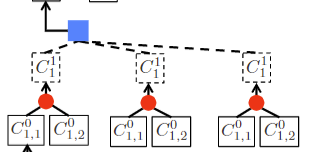
\includegraphics[width=0.4\linewidth]{figs/mult_attempts.png}
    \end{center}
    \item Given the probabilistic nature of creating GHZ states and the fusion operations, run these operations on multiple copies at each stage.
\end{itemize}
\end{frame}

\begin{frame}
    \frametitle{Building a Cluster State: Example}
    \textbf{\textbf{TODO:} make my own better figure of more relevant example}
    \begin{center}
        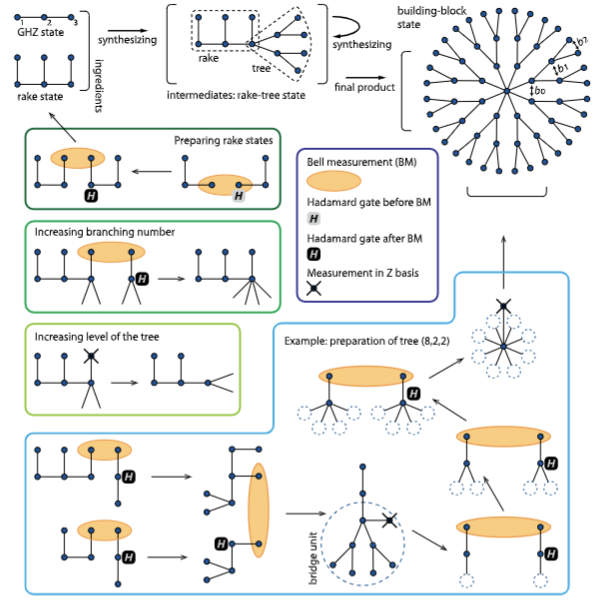
\includegraphics[width=0.5\linewidth]{figs/example_creation_stock.png}
    \end{center}
    \end{frame}

\begin{frame}
\frametitle{Naive Approach}
\begin{itemize}
    \item Build up the tree, through time steps.
    \item Each time step, combine states of similar size to create larger intermediate states.
    \begin{itemize}
        \item Each fusion step is attempted several times.
    \end{itemize}
    \item Start with GHZ states.
\end{itemize}
\begin{center}
    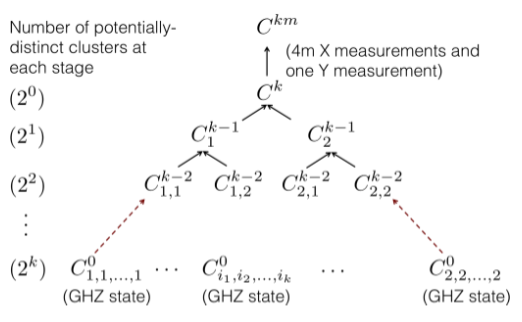
\includegraphics[width=0.5\linewidth]{figs/construction-overview.png}
\end{center}
\begin{itemize}
    \item \textbf{Problem:} If multiple attempts at a given fusion step succeed, then the other successful ones are wasted.
\end{itemize}
\end{frame}


\begin{frame}
\frametitle{Improved Approach}
\begin{itemize}
    \item \textbf{Solution:} Pool all the successful ones in a bank that any fusion step could pull from.
    \item Perform measurements early.
\end{itemize}
\begin{center}
    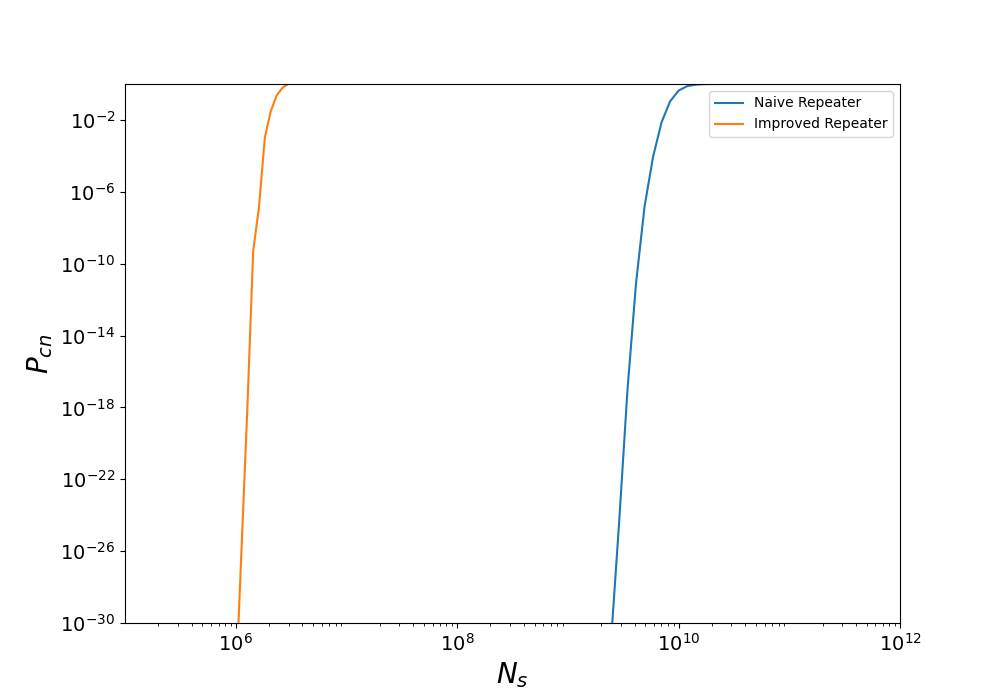
\includegraphics[width=0.65\linewidth]{figs/p_graph.png}
\end{center}
\end{frame}

\begin{frame}
    \frametitle{Rate Calculations}
    \begin{itemize}
        \item Key rate, in terms of bits per mode, is computed following formula below.
        \begin{align*}
            R = \frac{P_{cn} P_{meas}}{N_{parallel}}
        \end{align*}
        \item For improved scheme,
        \begin{equation}
            N_\text{parallel} = 2m
        \end{equation}
        \item For naive scheme,
        \begin{equation}
            N_\text{parallel} = 2m + 2m(b_0b_1 + b_0)
        \end{equation}
    \end{itemize}
    \end{frame}
    
    \begin{frame}
    \frametitle{Determining Loss Rates}
    \begin{itemize}
        \item For outer qubits, loss rate is given by:
        \begin{align*}
            \epsilon_{trav} = 1 - \eta^{1/(2n)}P_{chip}^{k+2}\eta_{GHZ}\eta_c
        \end{align*}
        \item For inner qubits, loss rate is given by:
        \begin{align*}
            \epsilon_{stat} = 1 - \eta^{1/n}P_{fib}P_{chip}^{k+2}\eta_{GHZ}\eta_c
        \end{align*}
    \end{itemize}
    \end{frame}
    
    \begin{frame}
    \frametitle{Determining Probabilities}
    \begin{itemize}
        \item Probability of an indriect $Z$ masurement at $i$th level, $\xi_i$ given by
        \begin{align*}
            \xi_i = 1 - [1- (1-\epsilon_{stat})(1-\epsilon_{stat}+\epsilon_{stat}\xi_{i+2})^{b_{i+1}}]^{b_i}, \text{ for } i \le \ell, 
            \xi_{\ell+1}=b_{\ell+1}=0.
        \end{align*}
        \item $P_X,P_Z$ is calculated as:
        \begin{align*}
           P_X &= 1 - [1-(1-\epsilon_{stat})^{b_1+1}]^{b_0} \\
            P_Z &= (1 - \epsilon_{stat}^{b_1+1})^{b_0} 
        \end{align*}
        \item Establish success rate of Bell state measurements:
        \begin{align*}
            P_B &= \left[\frac{1}{2}(\eta_s\eta_d)^2 + \frac{1}{4}(\eta_s\eta_d)^4\right] \cdot \left(P_{chip}^{k+2}\eta_{GHZ}\eta_c\right)^2 \cdot \eta^{1/n}
        \end{align*}
        \item Probability of at least one successful detection at ends is 
        \begin{equation*}
            P_{end} = 1 - (1-\eta^{1/(2n)}P_{chip}^{k+2}\eta_{GHZ}\eta_c)
        \end{equation*}
    \end{itemize}
    \end{frame}
    \begin{frame}
    \frametitle{Naive Approach Modifications}
    \begin{itemize}
        \item In naive approach, the number of parallel channels and success probability of Bell measurements change.
        \begin{align*}
            N_\text{parallel}&: 2m \rightarrow 2m + 2m(b_0b_1+b_0) \\ 
            P_\text{BSM}&: \frac{3}{4} \rightarrow \frac{1}{2} \\ 
            \epsilon&: \epsilon_\text{stat} \rightarrow \epsilon_\text{trav}
        \end{align*}
    \end{itemize}
    \begin{center}
        \centering
        \begin{tabular}{|c|c|c|c|c|c|c|}
            \hline
            $k$ & $m_\text{naive}$ & $\vec{b}_\text{naive}$ & $R_\text{naive}$ & $m_\text{improved}$ & $\vec{b}_\text{improved}$ & $R_\text{improved}$ \\
            \hline
            7   & 5                & $[3, 2]$              & $1.91 \times 10^{-8}$ & 4                   & $[4, 2]$                 & $3.87 \times 10^{-6}$ \\
            8   & 8                & $[4, 2]$              & $6.13 \times 10^{-6}$ & 5                   & $[5, 3]$                 & $2.98 \times 10^{-3}$ \\
            9   & 11               & $[5, 3]$              & $5.77 \times 10^{-4}$ & 7                   & $[6, 4]$                 & $2.71 \times 10^{-2}$ \\
            10  & 13               & $[7, 4]$              & $7.42 \times 10^{-4}$ & 8                   & $[10, 5]$                & $4.93 \times 10^{-2}$ \\
            \hline
        \end{tabular}
        \end{center}
    
    \end{frame}
    \begin{frame}
    \frametitle{Optimizing the number of repeater nodes}
    \begin{itemize}
        \item Optimal value of $n$ is different for each value of $L$
        \begin{center}
            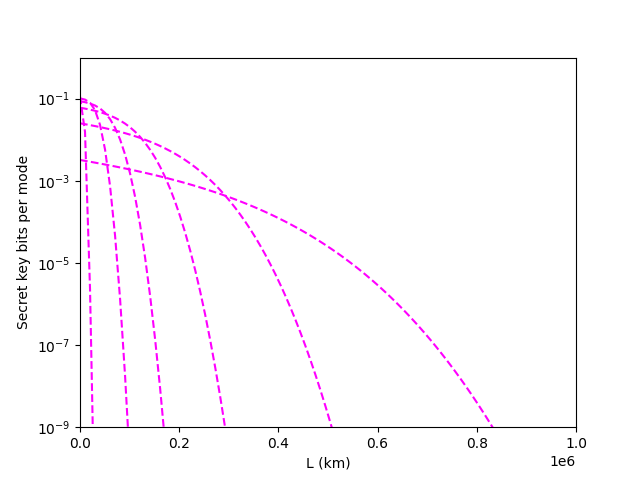
\includegraphics[width=0.5\linewidth]{figs/e_graph.png}
        \end{center}
        \item Satisfies the relationship 
        \begin{align*}
            \frac{L}{n} = 1.5\text{ km}.
        \end{align*}
    \end{itemize}
    \end{frame}
    \begin{frame}
    \frametitle{Comparison}
    \begin{itemize}
        \item Rate vs Distance for Naive (left) and Improved (right):
        \begin{center}
            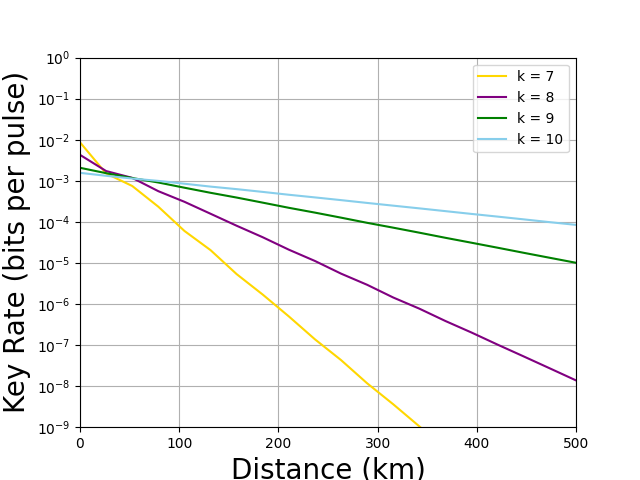
\includegraphics[width=0.49\linewidth]{figs/3a.png}
            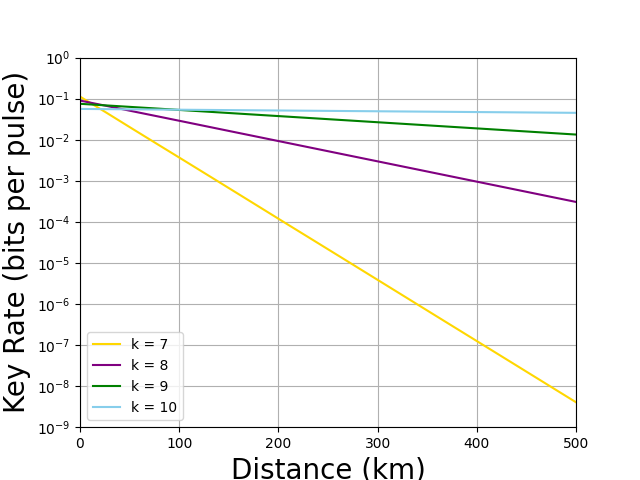
\includegraphics[width=0.49\linewidth]{figs/3b.png}
        \end{center}
    \end{itemize}
    \end{frame}
    
    \begin{frame}
    \Huge{\centerline{The End}}
    \end{frame}
    
    \end{document}